\newcommand{\F}{\mathbb{F}}
\newcommand{\C}{\mathbb{C}}
\newcommand{\an}{\mathscr{A}} 
\newcommand{\Q}{\mathbb{Q}}
\newcommand{\D}{\mathbb{D}}
\renewcommand{\hom}{\operatorname{Hom}}
\newcommand{\ehom}{\operatorname{End}}
\colorlet{gris}{black!60}

\-\vspace{-0.3cm}
  {\hrule \vspace{-0cm}
  \centering \textbf{Pós-P1 \ \(\mid\) \ Variável Complexa \ \(\mid\) \ \today} \vspace{0.2cm}
  \hrule
  Est. Nestor Aponte \ \(\mid\) \ RA 267452 \vspace{0.2cm}
  \hrule}

\vspace{0.5cm}
\textbf{Ex. 1.19.} Mostre que: \vspace{0.2cm}\\ 
(a) \(\sum nz^n\) não converge em nenhum ponto de \(\partial\D\).
\textcolor{gray}{
\[ |n|^{\nicefrac{1}{n}} = \exp (\nicefrac{1}{n}\cdot \log n ) \to \exp (0)  = 1\]  
Portanto, \(\sum nz^n < \infty\), se \(z \in \D\). Por outro lado, se \(|z| = 1\)
\[|n z^n| = n \cdot 1 = n \to \infty. \]
Em particular, \(nz^n \not\to 0\) e a série diverge.
}

(b) \(\sum \nicefrac{z^n}{n^2}\) converge em cada ponto de \(\partial \D\). 

\textcolor{gray}{
Pra cada \(z : |z|\leq 1\)  temos \(|f_n(z)| = |\nicefrac{1}{n^2} z^n| \leq \nicefrac{1}{n^2}\), como 
\[\sum_{n =1}^\infty \frac{1}{n^2} \leq \int_1^\infty \frac{1}{x^2} \ dx = \left(\lim_{x\to \infty} -\frac{1}{x}\right) - (-1)  = 1 < \infty,\]
pelo critério M-Weierstrass \(\sum f_n \overset{u}{\longrightarrow} f\) em todo \(\overline{\D}\). 
}

(c) \(\sum \nicefrac{z^n}{n}< \infty, \ \forall z \in \partial \D : z \neq 1\). Hint: somas parciais.
%\cite[cap. 1]{shakarchi} 

\textcolor{gray}{
A dica tem relação com um resultado mais geral conhecido como o Teste de Abel. Seja 
\[A_N := \sum^N_{n=1} z^n  + 1 - 1 = z \frac{1-z^N}{1-z}.\]
Para \(z \in \overline{\D}\setminus \{1\}\) fixo, \(|A_N| \leq \nicefrac{2}{|1-z|} =: C<  \infty\). Agora, 
\[S_N := \sum_{n=1}^N \frac{1}{n} \cdot z^n \overset{(?)}{=} \frac{1}{N}\cdot A_N + \sum^{N-1}_{n=1} A_n \left(\frac{1}{n}-\frac{1}{n+1}\right).\]
Tomando \(N\to \infty\) do módulo temos,  
\[|S_N| \leq C \frac{1}{N}  + C \left| 1 - \frac{1}{N} \right| \to  C< \infty,\]
isso pois após de tirar \(|A_n|\) fica série telescópica. Se \(z=1\) temos a série armônica \(\sum \nicefrac{1}{n} = \infty\).  
\vspace{0.3cm}
\hrule
\vspace{0.1cm}
\((?)\) Sendo \(a_n := z^n\) e \(b_n := \nicefrac{1}{n}\) note que,  \(-A_{j}b_{j+1} + A_{j+1} b_{j+1} = -A_jb_{j+1} + (A_j + a_{j+1}) b_{j+1} = a_{j+1}b_{j+1}\), logo
  %\sum^{N-1}_{n=1} A_n\left(b_n - b_{n+1}\right) = A_1b_1 -A_1b_2+ A_2b_2 -A_2b_3 + \cdots 
  \begin{align*}
    \sum^{N-1}_{n=1} A_n(b_n -b_{n+1}) &= A_1b_1 + \sum_{n=2}^{N-1}a_jb_j - A_{N-1}b_N \\ 
    &= \sum^{N-1}_{n=1} a_jb_j - (a_1 + \cdots + a_{N-1}) b_N
  \end{align*} 
  Finalmente somando o termo \(\nicefrac{1}{N}\cdot A_N = (a_1 + \cdots + a_N) b_N\) obtemos a fórmula utilizada acima. 
}

\newcommand{\M}{\mathcal{M}}
\textbf{Ex. 6.10.} Dada \(f: \R_+ \to \R\) contínua, a sua \emph{transformada de Mellin} é a função (complexa) dada por:
\[\M(f)(z) :=  \int_0^\infty f(t)\cdot t^{z-1} \ dt. \] 

(a) Mostre que para \(0 < \operatorname{Re}(z)< 1\), 
\begin{align*}
  \M(\cos)(z) &= \Gamma(z)\cdot \cos( \pi \cdot \nicefrac{ z}{2}) \text{ \ \  e} \\ 
  &\M(\sin)(z) = \Gamma(z)\cdot \sin( \pi \cdot\nicefrac{z}{2})
\end{align*}
Hint: Considere a integral da função \(f(w):= e^{-w} w^{z-1}\) no contorno descrito na seguinte figura,

\begin{textblock*}{6cm}(13.5cm, 4.5cm)
  \textcolor{black}{
  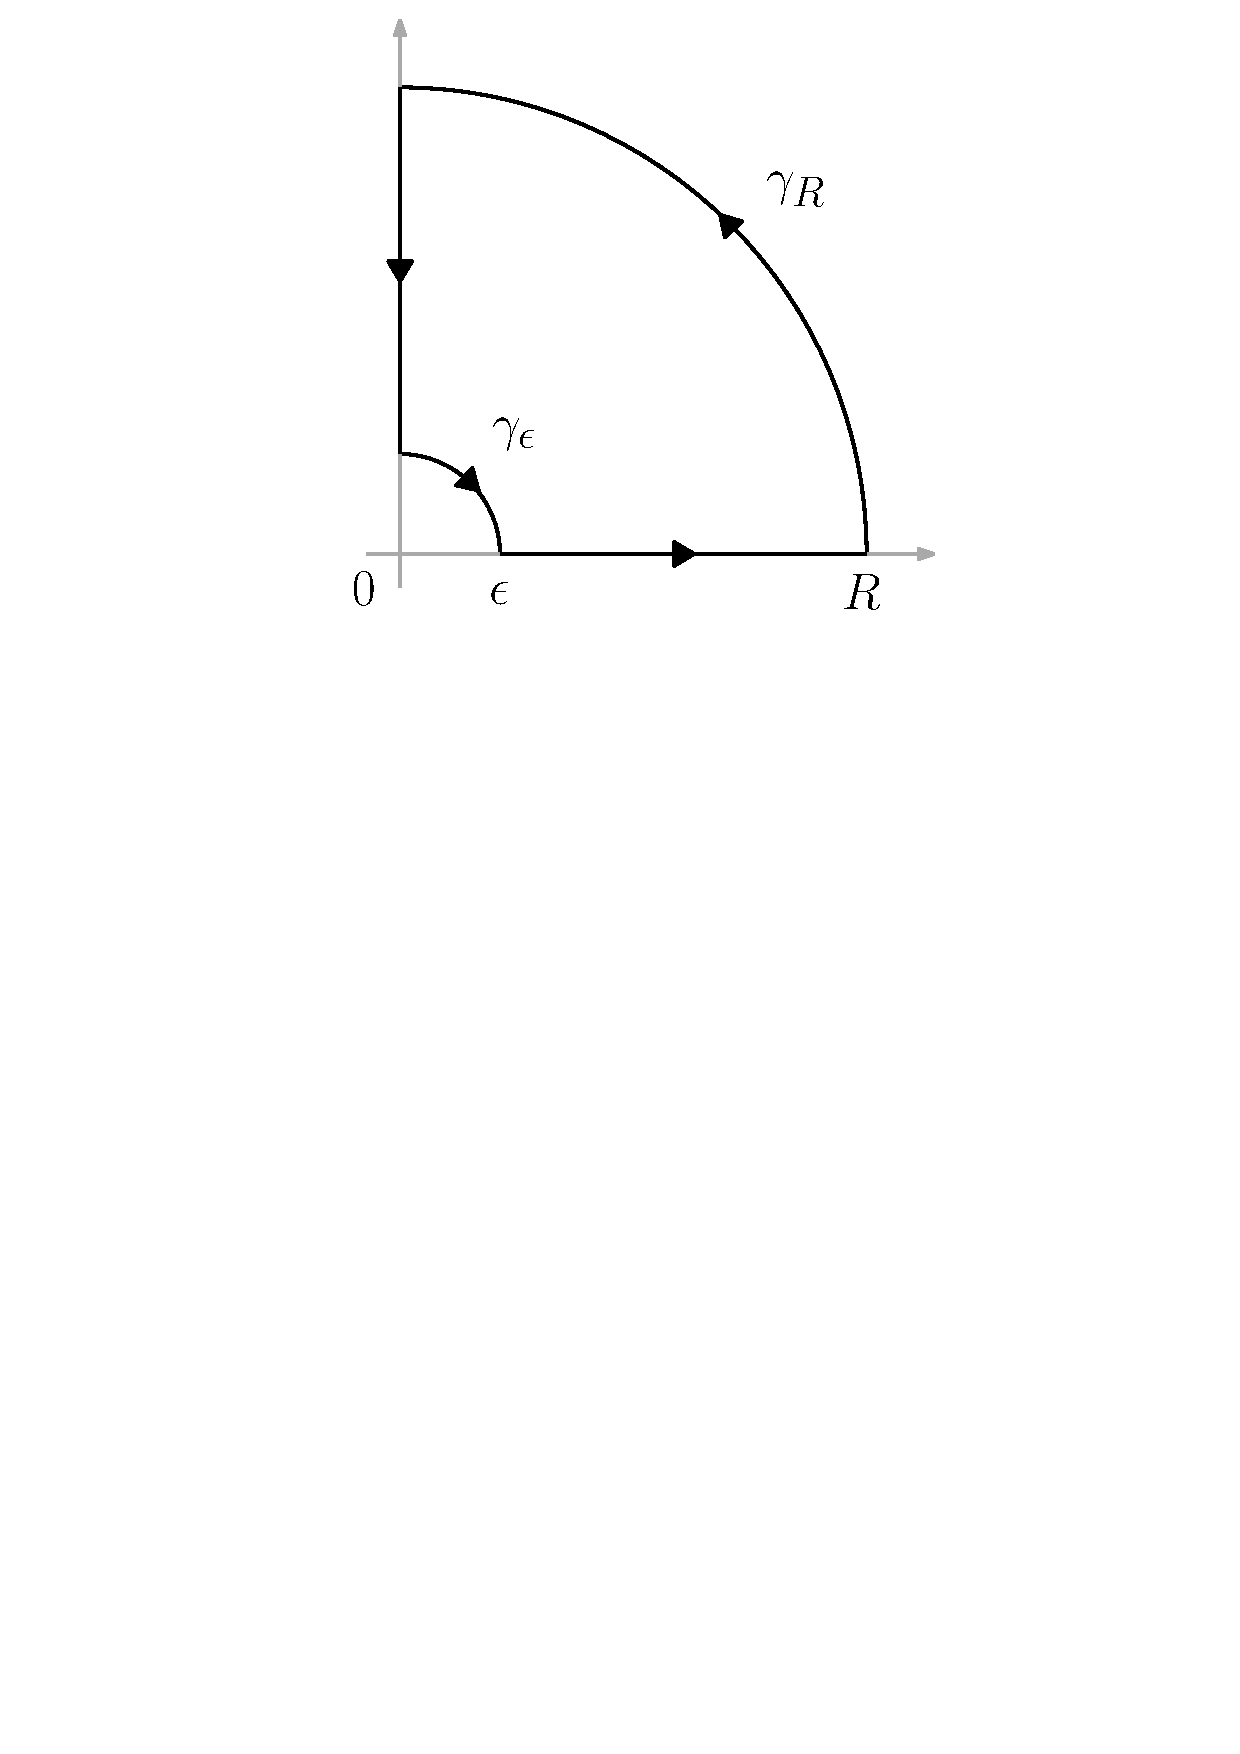
\includegraphics[width = 0.7\linewidth]{610.pdf}}
\end{textblock*}

\newcommand{\ho}{\mathcal{O}}
\vspace{5cm}
\textcolor{gray}{
  Seguindo a dica, chamemos de \(C\) a curva toda, \(f(w) = e^{-w} \exp ((z-1)\cdot \log w)\) é holomorfa em \(\C\setminus \{x \in \R : x \leq 0\}\), segue que do \(\blacksquare\) \hyperlink{thm222}{2.2. (\emph{Cauchy})} \cite[pag. 39]{shakarchi} que 
  \[\int_{C} f(w) \ dw = 0.\]   
  Como \(C = \gamma_\epsilon \cup [\epsilon, R] \cup \gamma_R \cup [iR, i\epsilon]\), vamos analizar cada uma dessas integrais, \(z = x+iy\).   
    \[\blacktriangleright \  \left|\int_{\gamma_\epsilon} f(w) \ dw\right| \leq \epsilon \cdot \frac{\pi}{2} \cdot \sup_{\gamma_\epsilon} |f| \to 0\]
    \vspace{-0.4cm}
    \begin{align*}
      \epsilon \cdot \sup_{\gamma_\epsilon} |e^{-w} w^{z-1}| &\leq \epsilon \cdot\sup_{\theta \in [0,\nicefrac{\pi}{2}]}|e^{-\epsilon \cos \theta}||\epsilon^{z-1}||e^{-\theta y}| \\ 
      &\leq \epsilon \cdot  M  \cdot| \epsilon^{x-1}|
    \end{align*}
    Pra \(0< \epsilon \ll 1\) a integral vai pra \(0\), sempre que \(x>0\). 
    \[\blacktriangleright \  \left|\int_{\gamma_R} f(w) \ dw\right| \leq M \cdot \left[\frac{R^{x-1}}{ e^R }e^{\nicefrac{2R\theta }{\pi}}\right]_0^{\nicefrac{\pi}{2}} \to 0 \]
    \begin{align*}
        \left|\int_{\gamma_R} (\cdots)\right| &\leq \int_0^{\nicefrac{\pi}{2}} |e^{-R\operatorname{cis(\theta)}} R^{z-1} e^{i\theta (z-1)} i R e^{i\theta} | \ d\theta  \\ 
      &\leq M \cdot R^{x}\int_0^{\nicefrac{\pi}{2}} e^{-R\cos \theta} \ d\theta  
      %& \leq M \cdot R^s \int_0^{\nicefrac{\pi}{2}} e^{\nicefrac{2R\theta}{\pi}}e^{-R} \ d\theta
    \end{align*}
    Como \(\ell(\theta):=  1 - \nicefrac{2\theta}{\pi}\leq \cos \theta, \ \theta \in [0, \nicefrac{\pi}{2}]\), temos \(e^{-R\cos \theta} \leq e^{-R\cdot\ell(\theta)}\), voltando 
    \begin{align*}
      \left|\int_{\gamma_R} (\cdots)\right| &\leq M \cdot \frac{R^x}{e^R}\int_0^{\nicefrac{\pi}{2}}e^{-\nicefrac{2R\theta }{\pi}} \ d\theta.
    \end{align*}
    Integrando obtemos a identidade acima e a integral vai pra \(0\) quando \(R \to \infty\) se \(x < 1\). 
    \vspace{0.2cm}
    \hrule 
    Após de fazer \(\epsilon \to 0\) e \(R\to \infty\) ficam então,  
    \begin{align*}
      \int_0^\infty e^{-t}t^{z-1} \ dt &= -\int_\infty^0 e^{-it} (it)^{z-1} \ i dt  \\ 
      &= i^z \int_0^\infty e^{-it} t^{z-1} \ dt  
    \end{align*}
    Como \(i^z = e^{z\cdot \log i} = e^{z \cdot (\log 1 + \operatorname{arg}i)} = e^{z\cdot \nicefrac{\pi}{2}} \) e lembrando que \(e^{i\theta} = \operatorname{cis}(\theta)\), obtemos que 
    \[\Gamma(z) \cdot \operatorname{cis}(-\pi \cdot \nicefrac{z}{2}) = \M(\cos)(z) - i \M(\sin)(z).\]
    Finalmente, igualando as partes real e imaginaria na igualdade acima obtemos as identidades do enunciado.
    }

    (b) Mostre que a fórmula do \(\M(\sin)(z)\) obtida no ítem (a) vale para \(|\operatorname{Re}(z)| < 1 \) e como conseqüência 

    \[\int_0^\infty \frac{\sin(x)}{x} \ dx = \frac{\pi}{2} \ \ \text{e} \ \ \int_0^\infty \frac{\sin(x)}{x^{\nicefrac{3}{2}}} \ dx = \sqrt{2\pi}. \]

    \textcolor{gray}{
      Olhemos primeiro pra a integral que define a transformada 
      \[\M(\sin)(z) = \int_0^\epsilon\sin(t)t^{z-1} \ dt + \int_\epsilon^\infty \sin(t) t^{z-1} \ dt\]
      %Perceba que para \(0 <t \ll 1, \ t^z \cdot \frac{\sin(t)}{t} \sim t^z\). Tambem, quanto a segunda integral conseguimos limitar com integrando monotono decrescente (convergente), logo  
      %\[\left|\int^\epsilon_0 t^z \ dt\right| \leq \int_0^\epsilon t^{x} \ dt  < \infty, \text{ \ se } x>-1\]
      %\[\left| \int_\epsilon^\infty \sin(t) t^{z-1} \ dt \right| \leq \left|\int_\epsilon^\infty t^{x-1} \ dt \right| < \infty,\ \text{ se } x < 1\]
      %Portanto a nossa integral toda converge se \(|\operatorname{Re}(z)|< 1\). 
      Sejam \(\{z\in \C : |\operatorname{Re}(z)|< 1\} =: \Omega\ab \subset \C\) e \(K\subset \Omega\) compacto, então \(\exists \delta > 0 : -1 + \delta \leq \operatorname{Re}(z) \leq 1 - \delta, \ \forall z\in K \). Como  \(|\sin(t) t^{z-1}| \leq t^{-\delta}\) se \(t\gg 1\) e \(|\sin(t) t^{z-1}| \sim |t^{z}| \leq t^{-1 + \delta}\) se \(0 <  t\ll 1 \), temos que pra \(z \in K\), 
      \[\int_0^1 (\cdots)  + \int_1^\infty (\cdots) \leq \int_0^1 t^{-1+\delta} \ dt + \int_1^\infty t^{-\delta} \ dt  < \infty\]
      Segue que a integral converge uniformemente em compactos dessa faixa. Pra \(t \in \R_+\) fixo o integrando é uma função inteira, assim pelo \(\blacksquare\) \hyperlink{thm33}{5.4.} \cite[pag. 56]{shakarchi} a integral define uma função holomorfa em \(\Omega\). Agora, \( \ho(\Omega)\ni \M(\sin)(z) = \Gamma(z) \sin(\pi \cdot \nicefrac{z}{2})\) em \(\{z\in \C : 0 < \operatorname{Re}(z)< 1\}\) conjunto com pontos de acumulação, segue do {\scriptsize\(\boxtimes\)} \hyperlink{coro33}{4.9.} \cite[pag. 52]{shakarchi} que as funções são idénticas em \(\Omega\). 
      \vspace{0.2cm}
      \hrule
      \vspace{-0.3cm}
      \begin{align*}
        \star \ \int_0^\infty \sin (x)\cdot x^{-1} \ dx &= \textstyle \underset{z \to 0}{\lim} \  \Gamma(z) \sin\left(\frac{\pi z}{2}\right) \\ 
        &\hspace{-1cm}= \textstyle \underset{z \to 0}{\lim} \ \left(\frac{1}{z} + o(1)\right) \left(\frac{\pi z}{2} - \frac{\pi^3z^3}{2^3 \cdot 3!} + \cdots \right) \\ 
        &\hspace{-0.5cm}= \textstyle \underset{z \to 0}{\lim} \ \left(\frac{\pi}{2} - \frac{\pi^3z^2}{2^3 \cdot 3!} + z\cdot o(1) \right) = \frac{\pi}{2}
      \end{align*}
      \vspace{-0.3cm}
      \begin{align*}
        \star \ \int_0^\infty \sin (x)\cdot x^{-\nicefrac{1}{2} - 1} \ dx &= \textstyle \Gamma\left(-\frac{1}{2}\right) \sin\left(\frac{-\nicefrac{\pi}{2}}{2}\right) \\ 
        &\overset{(?)}{=}\textstyle -2\cdot \Gamma\left(\frac{1}{2}\right) \left(\frac{-\sqrt{2}}{2}\right) = \sqrt{2\pi}  
      \end{align*}
      \hrule
      \vspace{-0.4cm}
      \[(?)\ \  \Gamma(-\nicefrac{1}{2} + 1) = -\nicefrac{1}{2} \cdot \Gamma(-\nicefrac{1}{2}) = \Gamma(\nicefrac{1}{2}) = \sqrt{\pi}.\] 
    }
